\documentclass[]{article}
\usepackage{graphicx}
\usepackage{placeins}
%opening
\title{Software Requirement Specification Document}
\author{Sandra Fares,Nour Ahmed ,Samiha Hesham, Mariam Hesham }

\begin{document}

\maketitle

\section{Introduction}

\subsection{Purpose of this document}
The main purpose of this document is to clarify and demonstrate the requirements of a Clinic System. These requirements include booking appointments, contacting Doctors or Physician assistants, and viewing patients' medical information. Our aim is to assist patients' to reserve appointments and reach out to healthcare professionals easily. Moreover, our system shall make it easier for Doctors to view patients' medical information, in order to provide accurate diagnosis. This documentation shall provide an explanation of each phase, along with an illustration on how this system is going to function. 

\subsection{ Scope of this document}
The scope of this document is to break down our client's problems into chunks that can be solved more readily.It also helps to increase understanding of issues and makes them easier to be tackled through our system and tested properly to fulfil the optimum solutions. 


\subsection{Overview}

The project clinic management is developed to facilitate the communication process between the doctor, the receptionist, the assistant and the patient. The software would be managed by two admins one is doctor and the other is receptionist. The doctor can view patient details and after checking up the patient, the recommended medicines for the patient are fed into the database by the doctor and are sent to receptionist. The patient can book an appointment and state the medical history .Receptionist would be responsible for viewing appointments and save it in the database along with their details .The receptionist can then generate bill and feed into the database. The system also maintains patient’s history so that doctor or assistant can view them anytime .The assistant would be responsible for booking an operation and follow up with the patient after the surgery .The system can thus reduce complexity in maintaining patient’s records.

\subsection{Business Context}

The project aims to build an application program to reduce the manual work for managing the clinic. It helps to end the complexities involved in accounting along with detailed profit and loss reports .The system can provide convenient access to information and making it less likely that mistakes would be made due to illegible writing. The internet-based access improves the ability to remotely access the data and making it easier to maintain and quicker to search through for relevant. The system also saves time for medical staff to focus on more important tasks at hand and reduces wait times which is otherwise spent filling out forms in and reduces the waiting time for patients at the clinics.


\section{General description}
\subsection{product functions}

\begin{enumerate}
  \item The system must be fully dynamic,in which the admin is fully controlling the system
  \item The users(patients,doctor,receptionists,assistants) must be able to control their information 
  \item The patient must be able to reserve his/her appointment online and choose either paying online or cash.
  \item The system should be able to send automatic emails and SMS to the patients.
  \item The admin should have full authority to control all staff permissions.
  \item The doctor must be able to see full information of the patient.
  \item The doctor should has the ability to write a report to the patient's case with all details.
  \item The doctor must be able to reserve operation for the patient if needed.
  \item The assistant must organize the doctor's schedule and add,edit or delete operations to it.
  \item The assistant should perform a broadcast en-forming patients of any cancellation in the doctor's schedule.
  \item The patients must have the authority to edit their appointment details.
  \item The receptionist must view patients' reservations and should deal with financial staff.
\end{enumerate}

\subsection{Similar System Information}
This software is similar to various generic products. However, MedDNA and eClinic are the most similar to our system. These systems are stand-alone clinic management systems that are available for installation by any customer in need. Their purpose is to help in managing appointments, viewing patients' history, and offering effortless communication between the Doctors and their Patients, just like our system is intended to do.


\subsection{ User Characteristics}
The admin, doctor, receptionists, assistants and patients will be the main users. The system is also designed to be user-friendly. 

\begin{itemize}
  \item Admin
  \item Receptionists
  \item Doctor
  \item Assistants
  \item Patients
  
  
\end{itemize}

Admin: Admin should have prior knowledge of the system. Admin is able to control the whole system. He/she can add, delete, update and modify the system.


Receptionists: in order view the details of the patients come for the treatment and accordingly provides identity to them also, schedule the appointments of the day and deals with payment methods. 


Doctor: Doctor should fairly know about the usage of the system. Doctor are able to see the respective appointments taken. And also, can view patient’s details and records and set for them operations if needed.


Assistants: they are mainly managing the chatting system for the clinic with patients and they must  view, edit ,delete and add operations in the doctor’s schedule.


Casual users: Anyone can view the information of the polyclinic. Patients can view their own records and doctor’s details and timings to take appointment online.


\subsection{ User Problem Statement}
Our client needs to replace all the manual operations done daily in his clinic into automated ones.Starting from patient's booking their appointments,saving their history to be easier to retrieve on the follow up day to booking surgeries too .Also they need a chatting system in order to facilitate patients contact with our client or his assistant .All of which should be easy to use , without any complexities to provide fast interactions without consuming time while dealing with our software.

\section{Functional Requirements}

\FloatBarrier
\begin{table}[h]
\caption{ }
\label{tab:my-table}
\begin{tabular}{|p{0.25\textwidth}|p{0.75\textwidth}|}
\hline
\textbf{Function:} & Check email validation.
\\ \hline
\textbf{ID}  &      FR00      

\\ \hline
\textbf{Description}    &    This Function is to check if the email is valid before inserting it in the database.                                                                 
\\ \hline
\textbf{Type}    &         Boolean

\\ \hline
\textbf{Input}        & Email


\\ \hline
\textbf{Action}            & Checks if the email entered in the text field  is in the proper format and  if the email is valid  it returns true means that the email is valid to be stored if exists in the database.

\\ \hline
\textbf{Output}            & Boolean if email is valid

\\ \hline
\textbf{Precondition}           &   User entered email into the required text field.

\\ \hline
\textbf{Post-condition}          & return to login function (FR03)  


\\ \hline
\textbf{Dependencies}           & return to login function (FR03).
\\ \hline
\end{tabular}
\end{table}

\FloatBarrier
\begin{table}[h]
\caption{ }
\label{tab:my-table}
\begin{tabular}{|p{0.25\textwidth}|p{0.75\textwidth}|}
\hline
\textbf{Function:} & Check password validation
\\ \hline
\textbf{ID}  &     FR01       

\\ \hline
\textbf{Description}    &      This Function is to check if the password is valid before inserting it in the database.                                                              
\\ \hline
\textbf{Type}    &         Boolean

\\ \hline
\textbf{Input}        & Password


\\ \hline
\textbf{Action}            & Checks if the password is valid in format. If yes it returns true means that the password is valid to be stored if exist in the database with its email.

\\ \hline
\textbf{Output}            & Boolean if password valid

\\ \hline
\textbf{Precondition}           &   User entered password into the required text field

\\ \hline
\textbf{Post-condition}           & Return to login function (FR03)


\\ \hline
\textbf{Dependencies}           & FR03
\\ \hline
\end{tabular}
\end{table}

\FloatBarrier
\begin{table}[h]
\caption{ }
\label{tab:my-table}
\begin{tabular}{|p{0.25\textwidth}|p{0.75\textwidth}|}
\hline
\textbf{Function:} & Check phone Number validation
\\ \hline
\textbf{ID}  &            FR02

\\ \hline
\textbf{Description}    &     This Function is to check if the phone number is valid before storing it in the database.                                                                
\\ \hline
\textbf{Type}    &       Boolean  

\\ \hline
\textbf{Input}        & Phone number


\\ \hline
\textbf{Action}            & Checks if the phone number entered in the  field  is in the proper format and  if it is valid in it's format it returns true means that it is valid to be stored in the database.

\\ \hline
\textbf{Output}            & Boolean if phone number is valid.

\\ \hline
\textbf{Precondition}           &   User enter the phone number into the required text field.

\\ \hline
\textbf{Post-condition}           & Return to login function (FR03)


\\ \hline
\textbf{Dependencies}           & FR03
\\ \hline
\end{tabular}
\end{table}

\FloatBarrier
\begin{table}[h]
\caption{ }
\label{tab:my-table}
\begin{tabular}{|p{0.25\textwidth}|p{0.75\textwidth}|}
\hline
\textbf{Function:} & Login.
\\ \hline
\textbf{ID}  &    FR03        

\\ \hline
\textbf{Description}    &       This Function is for the user to login into the system using his/her account.                                                              
\\ \hline
\textbf{Type}    &         Boolean

\\ \hline
\textbf{Input}        & Email and Password


\\ \hline
\textbf{Action}            & Checks if the data are filled and compare the record that was entered before to the record in the database, The function returns true otherwise returns false.

\\ \hline
\textbf{Output}            & Boolean acceptance login.

\\ \hline
\textbf{Precondition}           &   The user needs to into his email and password into the Text fields and that the inputs are verified (FR00, FR01)

\\ \hline
\textbf{Post-condition}           & Redirect to the home page


\\ \hline
\textbf{Dependencies}           & FR00, FR01
\\ \hline
\end{tabular}
\end{table}

\FloatBarrier
\begin{table}[h]
\caption{ }
\label{tab:my-table}
\begin{tabular}{|p{0.25\textwidth}|p{0.75\textwidth}|}
\hline
\textbf{Function:} & Forget Password
\\ \hline
\textbf{ID}  &            FR04

\\ \hline
\textbf{Description}    &       This Function exists if the user forgets the password, it generates a new password and sends email with it to help him login successfully again.                                                               
\\ \hline
\textbf{Type}    &       Boolean  

\\ \hline
\textbf{Input}        & Email


\\ \hline
\textbf{Action}            & Firstly the email is checked using FR00 then if the email exists in the database, the function sends email FR14 with the new password generated.

\\ \hline
\textbf{Output}            & Record updated

\\ \hline
\textbf{Precondition}           &   The user enters his email in the Text field.

\\ \hline
\textbf{Post-condition}     & Notification is sent to the user with new password.


\\ \hline
\textbf{Dependencies}           & FR00, FR14
\\ \hline
\end{tabular}
\end{table}


\FloatBarrier
\begin{table}[h]
\caption{}
\label{tab:my-table}
\begin{tabular}{|p{0.25\textwidth}|p{0.75\textwidth}|}
\hline
\textbf{Function:} & Create User.
\\ \hline
\textbf{ID}  & FR05          
\\ \hline
\textbf{Description}    &  The functions get the user type ID according from which page the inserting process whether the patient's registration page or from the administrator is happening, then it
uses the input data to insert a new row in users table in
the system database                                                              \\ \hline
\textbf{Type}    & void     
\\ \hline
\textbf{Input}  & user type id and user data
\\ \hline
\textbf{Action} &  checks if the user's email,password and phone number are validated, if so it enters the user record in the database and returns true else it returns false and an error message will appear 
\\ \hline
\textbf{Output} & New User Record in Database
\\ \hline
\textbf{Precondition}  & User's information is right and validated     
\\ \hline
\textbf{Post-condition} & Creating a new row in database table with new ID for the user
\\ \hline
\textbf{Dependencies} & FR00 , FR01 , FR02  
\\ \hline
\end{tabular}
\end{table}

\FloatBarrier
\begin{table}[h]
\caption{}
\label{tab:my-table}
\begin{tabular}{|p{0.25\textwidth}|p{0.75\textwidth}|}
\hline
\textbf{Function:} & Delete User.
\\ \hline
\textbf{ID}        &FR06            
\\ \hline
\textbf{Description} & The Function is to remove the selected user row from users table                                                         \\ \hline
\textbf{Type}     & Boolean       
\\ \hline
\textbf{Input}   & ID of the user selected to be removed 
\\ \hline
\textbf{Action}  & check if the user id exists in database
\\ \hline
\textbf{Output}  & A Success Message if User is deleted 
\\ \hline
\textbf{Precondition}  & Administrator chooses which user to be deleted  
\\ \hline
\textbf{Post-condition} & User Record is deleted from database and database is updated 
\\ \hline
\textbf{Dependencies}  &FR05 
\\ \hline
\end{tabular}
\end{table}

\FloatBarrier
\begin{table}[h]
\caption{}
\label{tab:my-table}
\begin{tabular}{|p{0.25\textwidth}|p{0.75\textwidth}|}
\hline
\textbf{Function:} & Search User.
\\ \hline
\textbf{ID}  & FR07           
\\ \hline
\textbf{Description} & The Function returns the user with the same id or name that being searched for by one of our staff users                                              
\\ \hline
\textbf{Type}  & Return Function        

\\ \hline
\textbf{Input}  & Id or Name of the desired user 

\\ \hline
\textbf{Action} & check if user id or name matches any of records in database , if there is a user show it else returns null
\\ \hline
\textbf{Output} & if Users details exists
\\ \hline
\textbf{Precondition}   &   One of staff users enters users id or name needed to be found
\\ \hline
\textbf{Post-condition} & user record is retrieved from database if is found 
\\ \hline
\textbf{Dependencies} & -- 
\\ \hline
\end{tabular}
\end{table}

\FloatBarrier
\begin{table}[h]
\caption{}
\label{tab:my-table}
\begin{tabular}{|p{0.25\textwidth}|p{0.75\textwidth}|}
\hline
\textbf{Function:} & Update User
\\ \hline
\textbf{ID}  &  FR08          
\\ \hline
\textbf{Description} & The Function performs an sql query to users table to update a certain record according to a specific user ID                                                     
\\ \hline
\textbf{Type}    &  Boolean       

\\ \hline
\textbf{Input}  & User ID and the desired category to be updated with it's new record  
\\ \hline
\textbf{Action} & check if those data can be updated 
\\ \hline
\textbf{Output}  & success message or failure message  
\\ \hline
\textbf{Precondition}  &  check if user exists in database and has the right to update 

\\ \hline
\textbf{Post-condition} & records in database are updated  
\\ \hline
\textbf{Dependencies}    & -- 
\\ \hline
\end{tabular}
\end{table}

\FloatBarrier
\begin{table}[h]
\caption{}
\label{tab:my-table}
\begin{tabular}{|p{0.25\textwidth}|p{0.75\textwidth}|}
\hline
\textbf{Function:} & Create Usertype
\\ \hline
\textbf{ID}  & FR09           

\\ \hline
\textbf{Description}  & this function is to add new user type to the system in the database                                                                     
\\ \hline
\textbf{Type}   & Boolean     

\\ \hline
\textbf{Input}  & User Type name

\\ \hline
\textbf{Action}  & Check if the user type name is not duplicated in the database , if so it enters the user type record in the database and returns true else return false

\\ \hline
\textbf{Output}  & Success Message if user type is created 

\\ \hline
\textbf{Precondition}  & Check if user type doesn't exist   
\\ \hline
\textbf{Post-condition}  & Creating a new database record with a new ID and add the new user type name in it 
\\ \hline
\textbf{Dependencies} & ---
\\ \hline
\end{tabular}
\end{table}
\FloatBarrier
\begin{table}[h]
\caption{}
\label{tab:my-table}
\begin{tabular}{|p{0.25\textwidth}|p{0.75\textwidth}|}
\hline
\textbf{Function:} & Update Usertype
\\ \hline
\textbf{ID}  & FR10          

\\ \hline
\textbf{Description} & this function is to Update an existing user type in database according to the user type ID \\ \hline
\textbf{Type}    &  Boolean       

\\ \hline
\textbf{Input}   & The User type data to be updated 

\\ \hline
\textbf{Action}  & Check if user type is updated and return true else return false or error message 

\\ \hline
\textbf{Output}  & Success Message if updated

\\ \hline
\textbf{Precondition}  & Check if user type exists    

\\ \hline
\textbf{Post-condition} & Update the system database row of the user type according to the user type ID  
\\ \hline
\textbf{Dependencies}  & FR09
\\ \hline
\end{tabular}
\end{table}

\FloatBarrier
\begin{table}[h]
\caption{}
\label{tab:my-table}
\begin{tabular}{|p{0.25\textwidth}|p{0.75\textwidth}|}
\hline
\textbf{Function:} & Delete UserType 
\\ \hline
\textbf{ID}  & FR11          

\\ \hline
\textbf{Description}  & This function is to delete the selected user type row from user type in database                                                                     
\\ \hline
\textbf{Type}   & Boolean         

\\ \hline
\textbf{Input}  & ID of which user type to be deleted 

\\ \hline
\textbf{Action} & Check if user Type id exists in the database to delete it 

\\ \hline
\textbf{Output}  & Message if user type deleted  

\\ \hline
\textbf{Precondition}   & The selected user type needed to be deleted   

\\ \hline
\textbf{Post-condition}  & Updating the database by removing the user type id row from table 

\\ \hline
\textbf{Dependencies}    & ---- 
\\ \hline
\end{tabular}
\end{table}

\FloatBarrier
\begin{table}[h]
\caption{}
\label{tab:my-table}
\begin{tabular}{|p{0.25\textwidth}|p{0.75\textwidth}|}
\hline
\textbf{Function:} & Indicates whether this class is abstract or concrete.
\\ \hline
\textbf{ID}  &            

\\ \hline
\textbf{Description}    &                                                                     
\\ \hline
\textbf{Type}    &         

\\ \hline
\textbf{Input}        & 


\\ \hline
\textbf{Action}            & 

\\ \hline
\textbf{Output}            & 

\\ \hline
\textbf{Precondition}           &   

\\ \hline
\textbf{Post-condition}           & 


\\ \hline
\textbf{Dependencies}           & 
\\ \hline
\end{tabular}
\end{table}

\FloatBarrier
\begin{table}[h]
\caption{Class Name - }
\label{tab:my-table}
\begin{tabular}{|p{0.25\textwidth}|p{0.75\textwidth}|}
\hline
\textbf{Function:} & Indicates whether this class is abstract or concrete.
\\ \hline
\textbf{ID}  &            

\\ \hline
\textbf{Description}    &                                                                     
\\ \hline
\textbf{Type}    &         

\\ \hline
\textbf{Input}        & 


\\ \hline
\textbf{Action}            & 

\\ \hline
\textbf{Output}            & 

\\ \hline
\textbf{Precondition}           &   

\\ \hline
\textbf{Post-condition}           & 


\\ \hline
\textbf{Dependencies}           & 
\\ \hline
\end{tabular}
\end{table}

\FloatBarrier
\begin{table}[h]
\caption{}
\label{tab:my-table}
\begin{tabular}{|p{0.25\textwidth}|p{0.75\textwidth}|}
\hline
\textbf{Function:} & Indicates whether this class is abstract or concrete.
\\ \hline
\textbf{ID}  &            

\\ \hline
\textbf{Description}    &                                                                     
\\ \hline
\textbf{Type}    &         

\\ \hline
\textbf{Input}        & 


\\ \hline
\textbf{Action}            & 

\\ \hline
\textbf{Output}            & 

\\ \hline
\textbf{Precondition}           &   

\\ \hline
\textbf{Post-condition}           & 


\\ \hline
\textbf{Dependencies}           & 
\\ \hline
\end{tabular}
\end{table}
\FloatBarrier
\begin{table}[h]
\caption{Class Name - }
\label{tab:my-table}
\begin{tabular}{|p{0.25\textwidth}|p{0.75\textwidth}|}
\hline
\textbf{Function:} & Add Appointment
\\ \hline
\textbf{ID}  &   FR15         

\\ \hline
\textbf{Description}    & This function adds a new record to the appointment table in the database                                                                    
\\ \hline
\textbf{Type}    &   Boolean      

\\ \hline
\textbf{Input}        & Appointment data to be recorded. Including the ID, Patient's ID, appointment number, type, and date.


\\ \hline
\textbf{Action}            & If the appointment is added successfully, it gets recorded in the database. else, it returns an error message.

\\ \hline
\textbf{Output}            & New appointment is added in the database

\\ \hline
\textbf{Precondition}           &  Patient books an appointment and fills up all the information needed to book an appointment. 

\\ \hline
\textbf{Post-condition}           & The appointment has been booked successfully and the patient is expected to meet his Doctor at the time he specified.


\\ \hline
\textbf{Dependencies}           & FR03, FR06 
\\ \hline
\end{tabular}
\end{table}


\FloatBarrier
\begin{table}[h]
\caption{Class Name - }
\label{tab:my-table}
\begin{tabular}{|p{0.25\textwidth}|p{0.75\textwidth}|}
\hline
\textbf{Function:} & Edit Appointment
\\ \hline
\textbf{ID}  & FR16    

\\ \hline
\textbf{Description}    &  This function updates the appointment data in the database according to the appointment ID.                                                                   
\\ \hline
\textbf{Type}    &  Boolean       

\\ \hline
\textbf{Input}        & Appointment ID to the appointment to be updated


\\ \hline
\textbf{Action}            & Checks if the appointment data has been updated. If yes, it returns true. else, it returns an error message.

\\ \hline
\textbf{Output}            & Appointment's data updated.

\\ \hline
\textbf{Precondition}           &   Checks if the appointment exists.

\\ \hline
\textbf{Post-condition}           & Update in the appointment table the selected appointment.


\\ \hline
\textbf{Dependencies}           &FR15 
\\ \hline
\end{tabular}
\end{table}

\FloatBarrier
\begin{table}[h]
\caption{Class Name - }
\label{tab:my-table}
\begin{tabular}{|p{0.25\textwidth}|p{0.75\textwidth}|}
\hline
\textbf{Function:} & Delete Appointment
\\ \hline
\textbf{ID}  &   FR17    

\\ \hline
\textbf{Description}    &   This function selects a specific row from the appointment table and removes it.                                                               
\\ \hline
\textbf{Type}    &     Boolean    

\\ \hline
\textbf{Input}        & ID for the desired appointment to be deleted.


\\ \hline
\textbf{Action}            & Checks if the appointment exists in the database. If yes, removes it. else, returns an error message.

\\ \hline
\textbf{Output}            & Appointment deleted successfully.

\\ \hline
\textbf{Precondition}           &   Checks if the appointment exists and select it.

\\ \hline
\textbf{Post-condition}           & Updating the database by removing the appointment row from the appointment table.

\\ \hline
\textbf{Dependencies}           & - 
\\ \hline
\end{tabular}
\end{table}

\FloatBarrier
\begin{table}[h]
\caption{Class Name - }
\label{tab:my-table}
\begin{tabular}{|p{0.25\textwidth}|p{0.75\textwidth}|}
\hline
\textbf{Function:} & Indicates whether this class is abstract or concrete.
\\ \hline
\textbf{ID}  &            

\\ \hline
\textbf{Description}    &                                                                     
\\ \hline
\textbf{Type}    &         

\\ \hline
\textbf{Input}        & 


\\ \hline
\textbf{Action}            & 

\\ \hline
\textbf{Output}            & 

\\ \hline
\textbf{Pre condition}           &   

\\ \hline
\textbf{Post condition}           & 


\\ \hline
\textbf{Dependncies}           & 
\\ \hline
\end{tabular}
\end{table}

\FloatBarrier
\begin{table}[h]
\caption{Class Name - }
\label{tab:my-table}
\begin{tabular}{|p{0.25\textwidth}|p{0.75\textwidth}|}
\hline
\textbf{Function:} & Indicates whether this class is abstract or concrete.
\\ \hline
\textbf{ID}  &            

\\ \hline
\textbf{Description}    &                                                                     
\\ \hline
\textbf{Type}    &         

\\ \hline
\textbf{Input}        & 


\\ \hline
\textbf{Action}            & 

\\ \hline
\textbf{Output}            & 

\\ \hline
\textbf{Pre condition}           &   

\\ \hline
\textbf{Post condition}           & 


\\ \hline
\textbf{Dependncies}           & 
\\ \hline
\end{tabular}
\end{table}

\FloatBarrier
\begin{table}[h]
\caption{Class Name - }
\label{tab:my-table}
\begin{tabular}{|p{0.25\textwidth}|p{0.75\textwidth}|}
\hline
\textbf{Function:} & Indicates whether this class is abstract or concrete.
\\ \hline
\textbf{ID}  &            

\\ \hline
\textbf{Description}    &                                                                     
\\ \hline
\textbf{Type}    &         

\\ \hline
\textbf{Input}        & 


\\ \hline
\textbf{Action}            & 

\\ \hline
\textbf{Output}            & 

\\ \hline
\textbf{Pre condition}           &   

\\ \hline
\textbf{Post condition}           & 


\\ \hline
\textbf{Dependncies}           & 
\\ \hline
\end{tabular}
\end{table}

\FloatBarrier
\begin{table}[h]
\caption{Class Name - }
\label{tab:my-table}
\begin{tabular}{|p{0.25\textwidth}|p{0.75\textwidth}|}
\hline
\textbf{Function:} & Indicates whether this class is abstract or concrete.
\\ \hline
\textbf{ID}  &            

\\ \hline
\textbf{Description}    &                                                                     
\\ \hline
\textbf{Type}    &         

\\ \hline
\textbf{Input}        & 


\\ \hline
\textbf{Action}            & 

\\ \hline
\textbf{Output}            & 

\\ \hline
\textbf{Pre condition}           &   

\\ \hline
\textbf{Post condition}           & 


\\ \hline
\textbf{Dependncies}           & 
\\ \hline
\end{tabular}
\end{table}

\FloatBarrier
\begin{table}[h]
\caption{Class Name - }
\label{tab:my-table}
\begin{tabular}{|p{0.25\textwidth}|p{0.75\textwidth}|}
\hline
\textbf{Function:} & Create Report
\\ \hline
\textbf{ID}  & FR22           

\\ \hline
\textbf{Description}    & This functions allows the Doctor to create or write reports to his patients if needed                                                                    
\\ \hline
\textbf{Type}    & String         

\\ \hline
\textbf{Input}        & Doctor specified and wrote a Diagnosis

\\ \hline
\textbf{Action}            & If the report is created successfully, it gets recorded in the database. else, it returns an error message  

\\ \hline
\textbf{Output}            & Report created successfully

\\ \hline
\textbf{Precondition}           & Doctor examines his patient and makes a Diagnosis

\\ \hline
\textbf{Post-condition}           & A new report is made for the patient and is successfully recorded in the database


\\ \hline
\textbf{Dependencies}           & FR03, FR06, FR15
\\ \hline
\end{tabular}
\end{table}

\FloatBarrier
\begin{table}[h]
\caption{Class Name - }
\label{tab:my-table}
\begin{tabular}{|p{0.25\textwidth}|p{0.75\textwidth}|}
\hline
\textbf{Function:} & Print Receipt
\\ \hline
\textbf{ID}  &  FR23        

\\ \hline
\textbf{Description}    &  This function prints a receipt for the patient of his booking fee and injection fee, if he needed any.                                                          
\\ \hline
\textbf{Type}    & float        

\\ \hline
\textbf{Input}  & Booking and/or injection fees


\\ \hline
\textbf{Action}            & If any payment is required, the function returns the overall fee for the patient if there is any. else, it returns an error message 

\\ \hline
\textbf{Output}            & Receipt containing the overall fee for the patient  

\\ \hline
\textbf{Precondition}           &  Patient books an appointment and/or uses an injection  

\\ \hline
\textbf{Post-condition}           & Printing successfully a receipt for the patient to review


\\ \hline
\textbf{Dependencies}           & FR03, FR15 
\\ \hline
\end{tabular}
\end{table}

\FloatBarrier
\begin{table}[h]
\caption{Class Name - }
\label{tab:my-table}
\begin{tabular}{|p{0.25\textwidth}|p{0.75\textwidth}|}
\hline
\textbf{Function:} & Add Operation
\\ \hline
\textbf{ID}  & FR24         

\\ \hline
\textbf{Description}    &  This function adds an operation by getting the operation ID according to which operation is being inserted and inserting it in the database                                                               
\\ \hline
\textbf{Type}    & void    

\\ \hline
\textbf{Input}        & The information needed for the operation such as, the operation's ID, location, date, hospital name, etc.


\\ \hline
\textbf{Action}            &  If the operation is added successfully, it is recorded in the database. else, it returns an error message

\\ \hline
\textbf{Output}            & New operation added to the database

\\ \hline
\textbf{Precondition}           &  Doctor examines the patient and determines that an operation must be made

\\ \hline
\textbf{Post-condition}           & An operation has been successfully recorded for the Doctor to perform


\\ \hline
\textbf{Dependencies}           & FR03, FR06, FR15
\\ \hline
\end{tabular}
\end{table}

\FloatBarrier
\begin{table}[h]
\caption{Class Name - }
\label{tab:my-table}
\begin{tabular}{|p{0.25\textwidth}|p{0.75\textwidth}|}
\hline
\textbf{Function:} & Edit Operation
\\ \hline
\textbf{ID}  &  FR25

\\ \hline
\textbf{Description}    &   This function updates the operation data in the database according to the operation ID                                                                  
\\ \hline
\textbf{Type}    &  Boolean       

\\ \hline
\textbf{Input}        & Operation ID to the operation to be updated


\\ \hline
\textbf{Action}            & Checks if the operation data has been updated. If yes, it returns true. else, it returns an error message 

\\ \hline
\textbf{Output}            & Operation's data updated

\\ \hline
\textbf{Precondition}           & Checks if the operation exists  

\\ \hline
\textbf{Post-condition}           & Update in the operation table the wanted operation


\\ \hline
\textbf{Dependencies}           & FR24
\\ \hline
\end{tabular}
\end{table}

\FloatBarrier
\begin{table}[h]
\caption{Class Name - }
\label{tab:my-table}
\begin{tabular}{|p{0.25\textwidth}|p{0.75\textwidth}|}
\hline
\textbf{Function:} & Delete Operation
\\ \hline
\textbf{ID}  &   FR26        

\\ \hline
\textbf{Description}    &  This function selects a specific row from the operation table and removes it.                                   
\\ \hline
\textbf{Type}    &   Boolean      

\\ \hline
\textbf{Input}        &  ID for the desired operation to be deleted 


\\ \hline
\textbf{Action}            & Checks if the operation exists in the database. If yes, removes it. else, returns an error message

\\ \hline
\textbf{Output}            & Operation deleted successfully 

\\ \hline
\textbf{Precondition}           & Checks if the operation exists and selects it

\\ \hline
\textbf{Post-condition}           & Updating the database by removing the operation row from the operation table


\\ \hline
\textbf{Dependencies}           & -
\\ \hline
\end{tabular}
\end{table}




\FloatBarrier
\section{Interface Requirements}
\bigskip
\subsection{User Interfaces}
\bigskip
\subsubsection {GUI}
 \bigskip
 \bigskip
\FloatBarrier
\subsubsection{Main page}
\vfill
\begin{figure}[h]
\centering
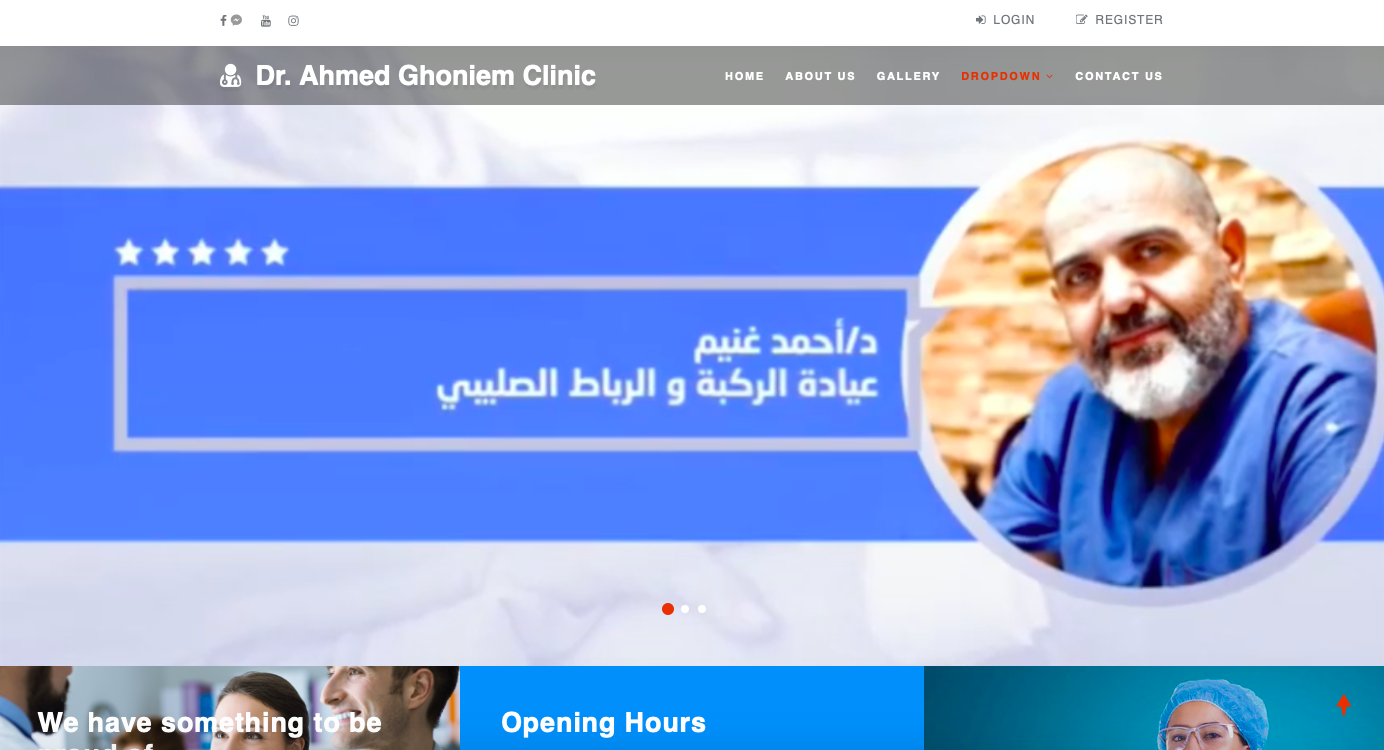
\includegraphics[width=10.0cm, height=10.0cm]{./Home.png}
\caption{Main Page of website the patient use it}
\label{label1}
\end{figure}
\vfill
\newpage
\FloatBarrier
\subsubsection{Login pages}
\FloatBarrier
\begin{figure}[h]
\centering
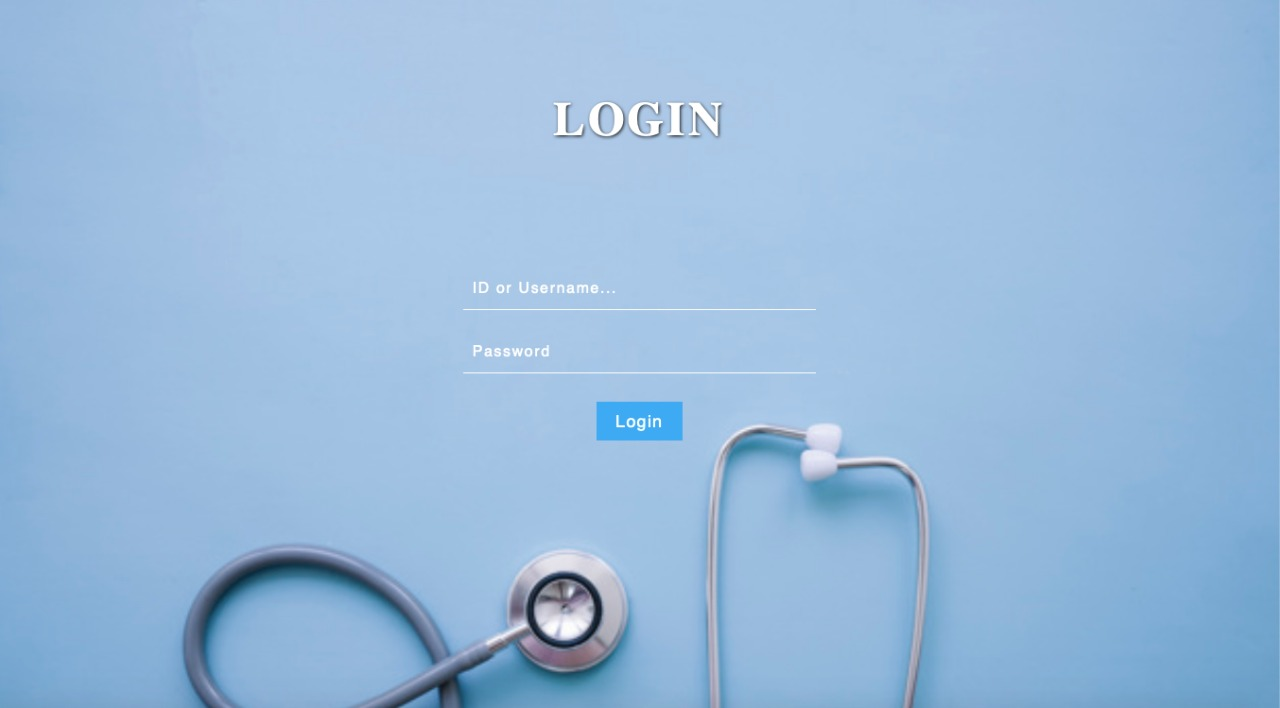
\includegraphics[width=10.0cm, height=10.0cm]{./2.jpeg}
\caption{Staff's Login}
\label{label1}
\end{figure}
\begin{figure}[h]
\centering
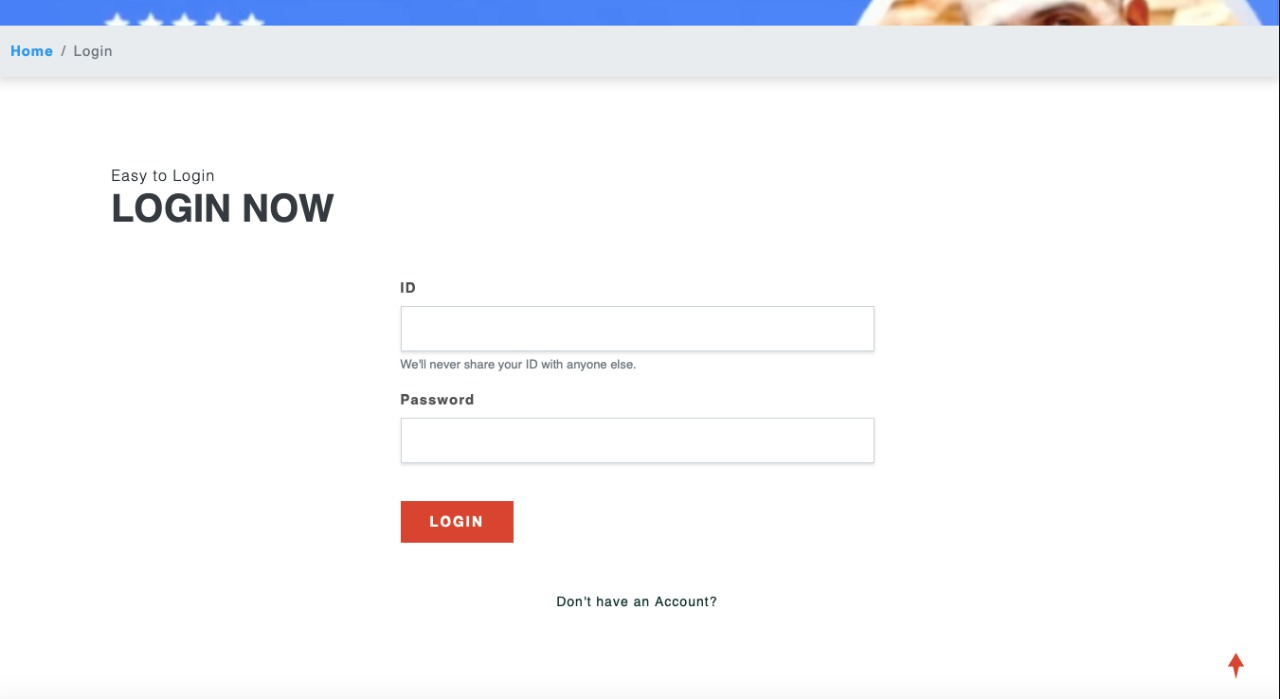
\includegraphics[width=10.0cm, height=10.0cm]{./3.jpeg}
\caption{Patient's login}
\label{label2}
\end{figure}
\FloatBarrier
\bigskip
\bigskip
\subsubsection{Patient's Registration}
\begin{figure}
 \begin{minipage}{.5\textwidth}
  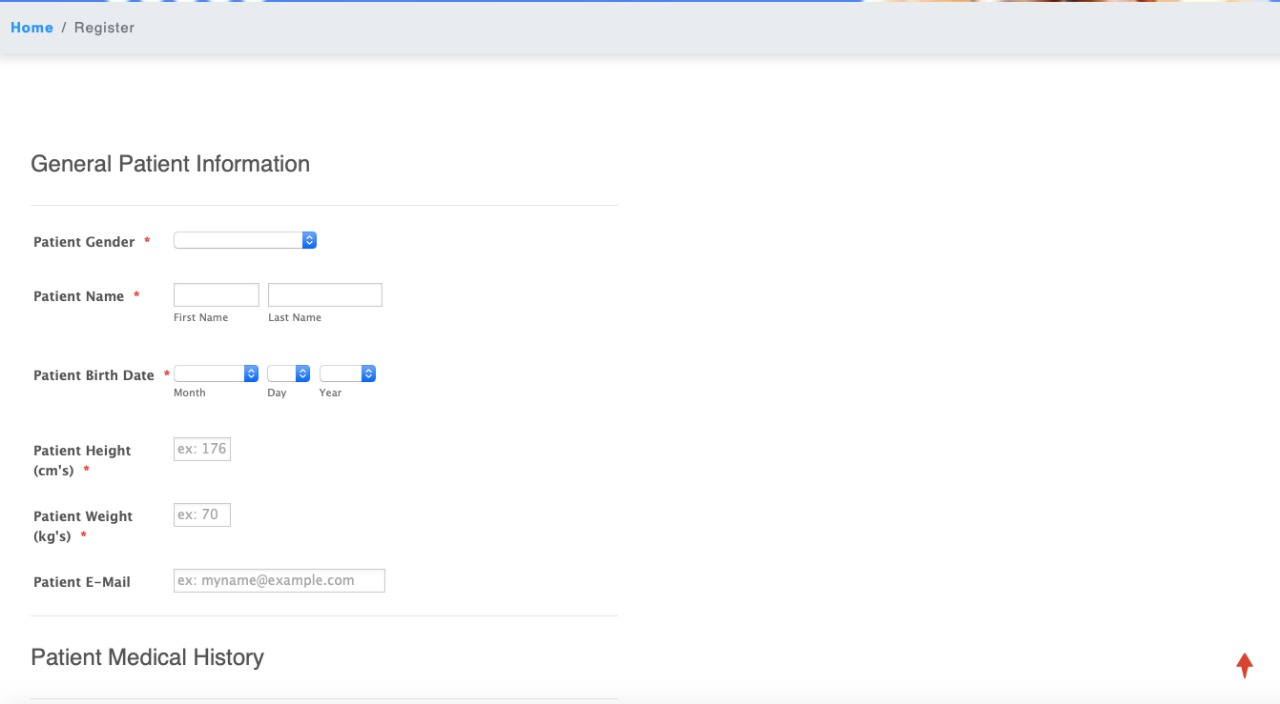
\includegraphics[width=8.0cm, height=8.0cm]{./reg1.jpeg}
  \caption{1}
 \end{minipage}
 \begin{minipage}{.5\textwidth}
  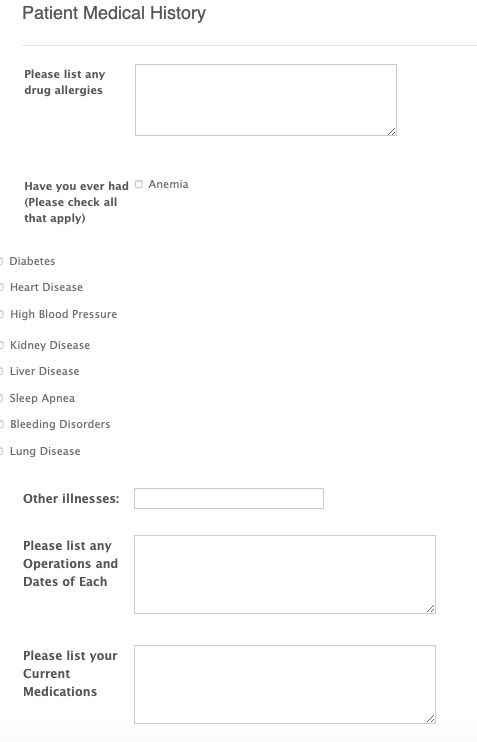
\includegraphics[width=8.0cm, height=8.0cm]{./reg2.jpeg}
  \caption{2}
 \end{minipage}
  \begin{minipage}{.5\textwidth}
  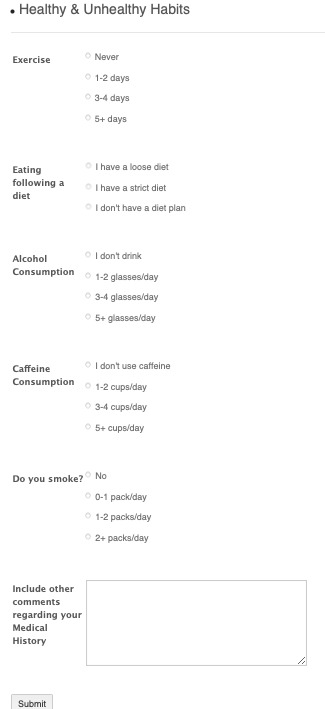
\includegraphics[width=8.0cm, height=8.0cm]{./reg3.jpeg}
  \caption{3}
 \end{minipage}
\end{figure}
\FloatBarrier
\FloatBarrier
\subsubsection{Doctor's Dashboard}
\begin{figure}[h]
\centering
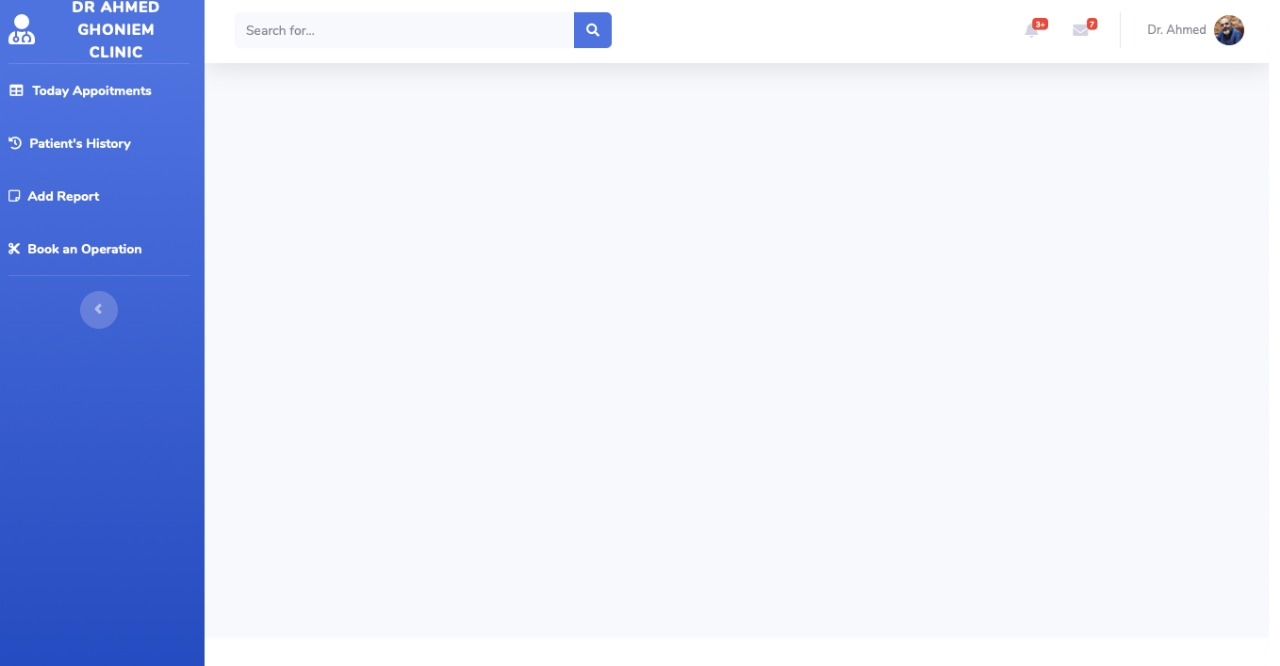
\includegraphics[width=10.0cm, height=10.0cm]{./Dr.png}
\caption{Doctor's dashboard}
\label{label1}
\end{figure}
\FloatBarrier
\newpage
\FloatBarrier
\subsubsection{Booking Page}
\begin{figure}[h]
\centering
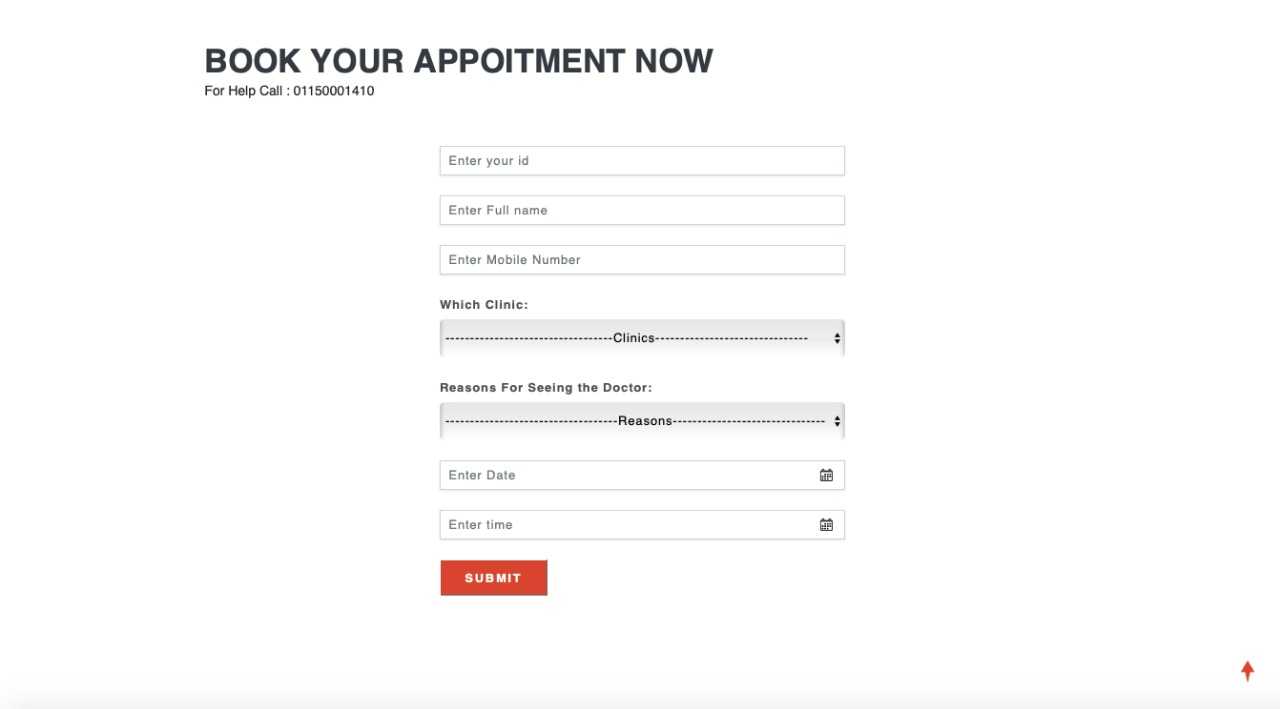
\includegraphics[width=15.5cm, height=10.0cm]{./b1.jpeg}
\caption{Booking Page}
\label{label1}
\end{figure}
\FloatBarrier
\newpage
\FloatBarrier
\subsubsection{Appointment's Time Table Page}
\begin{figure}[h]
\centering
\includegraphics[width=15.5cm, height=10.0cm]{./time.jpeg}
\caption{Appointment Page}
\label{label1}
\end{figure}
\FloatBarrier

\subsubsection { CLI}
N/A

\subsection {API}
N/A


\section{Design Constraints}
The system should be adaptable to be vied from different kinds of devices
either tablets, laptops... etc. Also we had a constrain with which is the
internet speed it varies from one user to another. 
\section{Other non-functional attributes}


\subsection {Security}
This system is provided with authentication without which no user can pass. So only the legitimate users are allowed to use the application. If the legitimate user’s share the authentication information then the system is open to outsiders.



\subsection {Reliability}
Good validations of user inputs will be done to avoid incorrect storage of records.
\subsection {Maintainability}



\subsection {Portability}
This system can be installed in any personal computers supporting windows operating system platform.
\subsection {Flexibility}
The system keeps on updating the data according to the transactions that takes place.

\section{Preliminary Object-Oriented Domain Analysis}
This section presents a list of the fundamental objects that must be modeled within the system to satisfy its requirements. The purpose is to provide an alternative, ''structural'' view on the requirements stated above and how they might be satisfied in the system. A primitive class diagram to be delivered.

\subsection{Class diagram}
This section should contain a set of graphs that illustrate the primary inheritance hierarchy (is-kind-of) for the system. For example: 



\subsection{ER diagram}
This section presents a more detailed description of each class identified during the OO Domain Analysis.
Each class description should conform to the following structure: 



\section{Operational Scenarios}
use case diagram

\section{Project Plan}
\FloatBarrier
\begin{table}[h]
\caption{}
\label{tab:my-table}
\begin{tabular}{|p{0.5\textwidth}|p{0.5\textwidth}|}
\hline
\textbf{Task} & \textbf{End Date}
\\ \hline
\textbf{Html templates}  & 17/3/2020            

\\ \hline
\textbf{UserInterface }  &  17/3/2020                          
\\ \hline
\textbf{Booking Interface}  & 17/3/2020
\\ \hline
\textbf{User Full Control}  &  4/4/2020  
\\ \hline
\textbf{Staff Full Control}  &  10/4/2020  

\\ \hline
\textbf{Booking Full Control} & 10/4/2020

\\ \hline
\textbf{Messaging}   & 15/4/2020

\\ \hline
\textbf{Project Full Control} & 5/5/2020

\\ \hline
\end{tabular}
\end{table}


\subsection{ Abbreviations}
\begin{itemize}

\item SMS = Short Message Service
\item ER=Entity Relationship diagram

\end{itemize}


\FloatBarrier
\subsection{Collected material}


\begin{figure}[h]
\centering
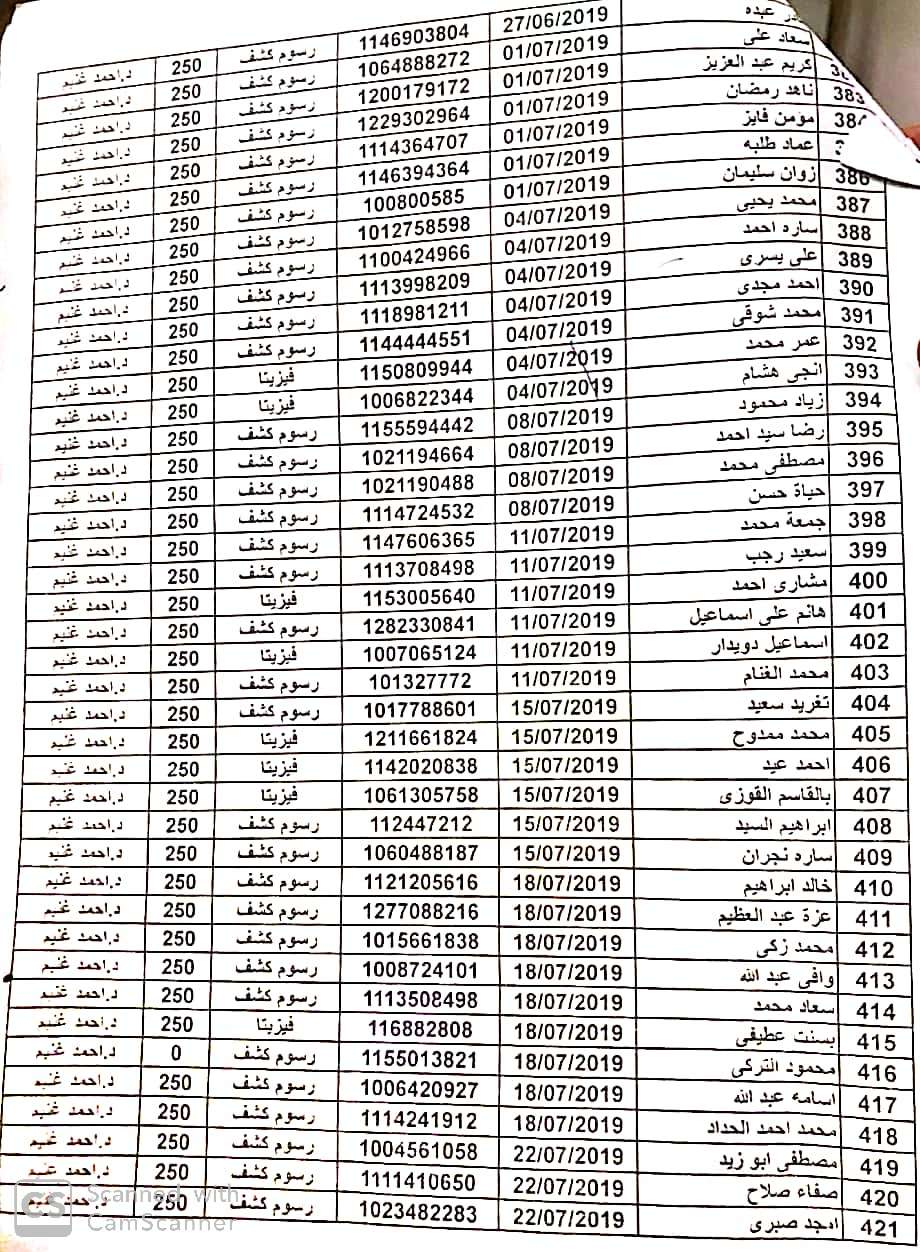
\includegraphics[width=10.0cm, height=10.0cm]{./ref1.jpeg}
\label{label1}
\end{figure}
\begin{figure}[h]
\centering
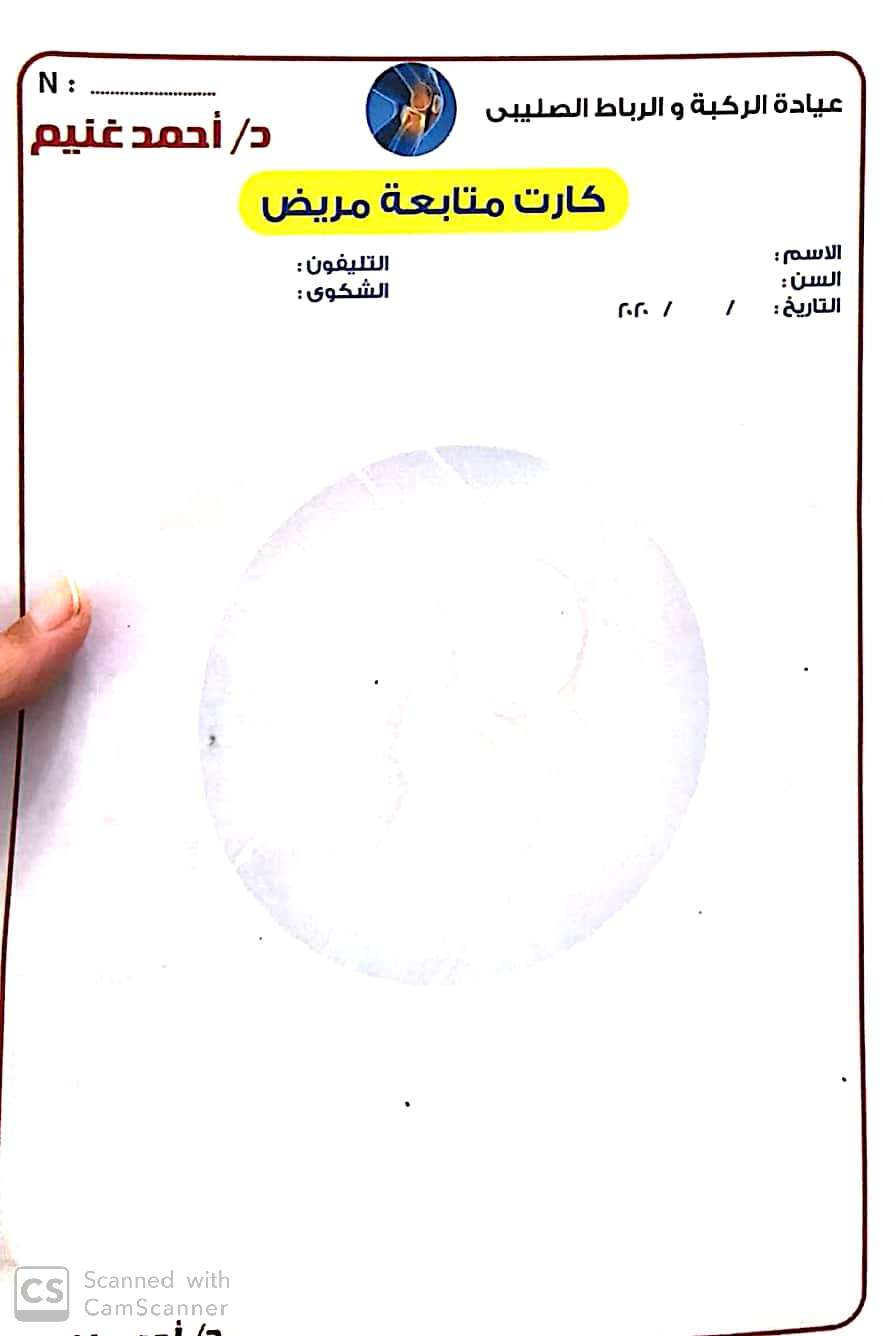
\includegraphics[width=10.0cm, height=10.0cm]{./ref2.jpeg}

\label{label2}
\end{figure}
\FloatBarrier

\section {References}

\bibliographystyle{IEEEtranS}

\bibliography{cite}

\end{document}
